

\documentclass[journal,12pt,twocolumn]{IEEEtran}
\usepackage{setspace}
\usepackage{gensymb}
\usepackage{caption}
%\usepackage{multirow}
%\usepackage{multicolumn}
%\usepackage{subcaption}
%\doublespacing
\singlespacing
\usepackage{csvsimple}
\usepackage{amsmath}
\usepackage{multicol}
%\usepackage{enumerate}
\usepackage{amssymb}
%\usepackage{graphicx}
\usepackage{newfloat}
%\usepackage{syntax}
\usepackage{listings}
\usepackage{color}
\usepackage{tikz}
\usepackage{graphicx}
\usetikzlibrary{shapes,arrows}

%\usepackage{graphicx}
%\usepackage{amssymb}
%\usepackage{relsize}
%\usepackage[cmex10]{amsmath}
%\usepackage{mathtools}
%\usepackage{amsthm}
%\interdisplaylinepenalty=2500
%\savesymbol{iint}
%\usepackage{txfonts}
%\restoresymbol{TXF}{iint}
%\usepackage{wasysym}
\usepackage{amsthm}
\usepackage{mathrsfs}
\usepackage{txfonts}
\usepackage{stfloats}
\usepackage{cite}
\usepackage{cases}
\usepackage{mathtools}
\usepackage{caption}
\usepackage{enumerate}	
\usepackage{enumitem}
\usepackage{amsmath}
%\usepackage{xtab}
\usepackage{longtable}
\usepackage{multirow}
%\usepackage{algorithm}
%\usepackage{algpseudocode}
\usepackage{enumitem}
\usepackage{mathtools}
\usepackage{hyperref}
%\usepackage[framemethod=tikz]{mdframed}
\usepackage{listings}
    %\usepackage[latin1]{inputenc}                                 %%
    \usepackage{color}                                            %%
    \usepackage{array}                                            %%
    \usepackage{longtable}                                        %%
    \usepackage{calc}                                             %%
    \usepackage{multirow}                                         %%
    \usepackage{hhline}                                           %%
    \usepackage{ifthen}                                           %%
  %optionally (for landscape tables embedded in another document): %%
    \usepackage{lscape}     


\usepackage{url}
\def\UrlBreaks{\do\/\do-}


%\usepackage{stmaryrd}


%\usepackage{wasysym}
%\newcounter{MYtempeqncnt}
\DeclareMathOperator*{\Res}{Res}
%\renewcommand{\baselinestretch}{2}
\renewcommand\thesection{\arabic{section}}
\renewcommand\thesubsection{\thesection.\arabic{subsection}}
\renewcommand\thesubsubsection{\thesubsection.\arabic{subsubsection}}

\renewcommand\thesectiondis{\arabic{section}}
\renewcommand\thesubsectiondis{\thesectiondis.\arabic{subsection}}
\renewcommand\thesubsubsectiondis{\thesubsectiondis.\arabic{subsubsection}}

% correct bad hyphenation here
\hyphenation{op-tical net-works semi-conduc-tor}

%\lstset{
%language=C,
%frame=single, 
%breaklines=true
%}

%\lstset{
	%%basicstyle=\small\ttfamily\bfseries,
	%%numberstyle=\small\ttfamily,
	%language=Octave,
	%backgroundcolor=\color{white},
	%%frame=single,
	%%keywordstyle=\bfseries,
	%%breaklines=true,
	%%showstringspaces=false,
	%%xleftmargin=-10mm,
	%%aboveskip=-1mm,
	%%belowskip=0mm
%}

%\surroundwithmdframed[width=\columnwidth]{lstlisting}
\def\inputGnumericTable{}                                 %%
\lstset{
%language=C,
frame=single, 
breaklines=true,
columns=fullflexible
}
\begin{document}

%


\newtheorem{theorem}{Theorem}[section]
\newtheorem{problem}{Problem}
\newtheorem{proposition}{Proposition}[section]
\newtheorem{lemma}{Lemma}[section]
\newtheorem{corollary}[theorem]{Corollary}
\newtheorem{example}{Example}[section]
\newtheorem{definition}[problem]{Definition}
%\newtheorem{thm}{Theorem}[section] 
%\newtheorem{defn}[thm]{Definition}
%\newtheorem{algorithm}{Algorithm}[section]
%\newtheorem{cor}{Corollary}
\newcommand{\BEQA}{\begin{eqnarray}}
\newcommand{\EEQA}{\end{eqnarray}}
\newcommand{\define}{\stackrel{\triangle}{=}}
\newcommand*\circled[1]{\tikz[baseline=(char.base)]{
    \node[shape=circle,draw,inner sep=2pt] (char) {#1};}}
\bibliographystyle{IEEEtran}
%\bibliographystyle{ieeetr}
\providecommand{\mbf}{\mathbf}
\providecommand{\pr}[1]{\ensuremath{\Pr\left(#1\right)}}
\providecommand{\qfunc}[1]{\ensuremath{Q\left(#1\right)}}
\providecommand{\sbrak}[1]{\ensuremath{{}\left[#1\right]}}
\providecommand{\lsbrak}[1]{\ensuremath{{}\left[#1\right.}}
\providecommand{\rsbrak}[1]{\ensuremath{{}\left.#1\right]}}
\providecommand{\brak}[1]{\ensuremath{\left(#1\right)}}
\providecommand{\lbrak}[1]{\ensuremath{\left(#1\right.}}
\providecommand{\rbrak}[1]{\ensuremath{\left.#1\right)}}
\providecommand{\cbrak}[1]{\ensuremath{\left\{#1\right\}}}
\providecommand{\lcbrak}[1]{\ensuremath{\left\{#1\right.}}
\providecommand{\rcbrak}[1]{\ensuremath{\left.#1\right\}}}
\theoremstyle{remark}
\newtheorem{rem}{Remark}
\newcommand{\sgn}{\mathop{\mathrm{sgn}}}
\providecommand{\fourier}{\overset{\mathcal{F}}{ \rightleftharpoons}}
%\providecommand{\hilbert}{\overset{\mathcal{H}}{ \rightleftharpoons}}
\providecommand{\system}{\overset{\mathcal{H}}{ \longleftrightarrow}}
	%\newcommand{\solution}[2]{\textbf{Solution:}{#1}}
\newcommand{\solution}{\noindent \textbf{Solution: }}
\newcommand{\cosec}{\,\text{cosec}\,}
\providecommand{\dec}[2]{\ensuremath{\overset{#1}{\underset{#2}{\gtrless}}}}
\newcommand{\myvec}[1]{\ensuremath{\begin{pmatrix}#1\end{pmatrix}}}
\newcommand{\mydet}[1]{\ensuremath{\begin{vmatrix}#1\end{vmatrix}}}
%\numberwithin{equation}{section}
%\numberwithin{figure}{section}
%\numberwithin{table}{section}
%\numberwithin{equation}{subsection}
%\numberwithin{problem}{section}
%\numberwithin{definition}{section}
\makeatletter
\@addtoreset{figure}{problem}
\makeatother
\let\StandardTheFigure\thefigure
\let\vec\mathbf
%\renewcommand{\thefigure}{\theproblem.\arabic{figure}}
\renewcommand{\thefigure}{\theproblem}
%\setlist[enumerate,1]{before=\renewcommand\theequation{\theenumi.\arabic{equation}}
%\counterwithin{equation}{enumi}
%\renewcommand{\theequation}{\arabic{subsection}.\arabic{equation}}
\def\putbox#1#2#3{\makebox[0in][l]{\makebox[#1][l]{}\raisebox{\baselineskip}[0in][0in]{\raisebox{#2}[0in][0in]{#3}}}}
     \def\rightbox#1{\makebox[0in][r]{#1}}
     \def\centbox#1{\makebox[0in]{#1}}
     \def\topbox#1{\raisebox{-\baselineskip}[0in][0in]{#1}}
     \def\midbox#1{\raisebox{-0.5\baselineskip}[0in][0in]{#1}}
\title{
	%\logo{
%Computational Approach to School Geometry
	Assignment
%	}
}
\author{ Pettugadi Pranav\\CS21BTECH11063% <-this % stops a space
}	
%\title{
%	\logo{Matrix Analysis through Octave}{\begin{center}\includegraphics[scale=.24]{tlc}\end{center}}{}{HAMDSP}
%}
% paper title
% can use linebreaks \\ within to get better formatting as desired
%\title{Matrix Analysis through Octave}
%
%
% author names and IEEE memberships
% note positions of commas and nonbreaking spaces ( ~ ) LaTeX will not break
% a structure at a ~ so this keeps an author's name from being broken across
% two lines.
% use \thanks{} to gain access to the first footnote area
% a separate \thanks must be used for each paragraph as LaTeX2e's \thanks
% was not built to handle multiple paragraphs
%
%\author{<-this % stops a space
%\thanks{}}
%}
% note the % following the last \IEEEmembership and also \thanks - 
% these prevent an unwanted space from occurring between the last author name
% and the end of the author line. i.e., if you had this:
% 
% \author{....lastname \thanks{...} \thanks{...} }
%                     ^------------^------------^----Do not want these spaces!
%
% a space would be appended to the last name and could cause every name on that
% line to be shifted left slightly. This is one of those "LaTeX things". For
% instance, "\textbf{A} \textbf{B}" will typeset as "A B" not "AB". To get
% "AB" then you have to do: "\textbf{A}\textbf{B}"
% \thanks is no different in this regard, so shield the last } of each \thanks
% that ends a line with a % and do not let a space in before the next \thanks.
% Spaces after \IEEEmembership other than the last one are OK (and needed) as
% you are supposed to have spaces between the names. For what it is worth,
% this is a minor point as most people would not even notice if the said evil
% space somehow managed to creep in.
%\WarningFilter{latex}{LaTeX Warning: You have requested, on input line 117, version}
% The paper headers
%\markboth{Journal of \LaTeX\ Class Files,~Vol.~6, No.~1, January~2007}%
%{Shell \MakeLowercase{\textit{et al.}}: Bare Demo of IEEEtran.cls for Journals}
% The only time the second header will appear is for the odd numbered pages
% after the title page when using the twoside option.
% 
% * Note that you probably will NOT want to include the author's *
% * name in the headers of peer review papers.                   *
% You can use \ifCLASSOPTIONpeerreview for conditional compilation here if
% you desire.
% If you want to put a publisher's ID mark on the page you can do it like
% this:
%\IEEEpubid{0000--0000/00\$00.00~\copyright~2007 IEEE}
% Remember, if you use this you must call \IEEEpubidadjcol in the second
% column for its text to clear the IEEEpubid mark.
% make the title area
\maketitle

\tableofcontents

\bigskip

\renewcommand{\thefigure}{\theenumi}
\renewcommand{\thetable}{\theenumi}
%\renewcommand{\theequation}{\theenumi}
%\begin{abstract}
%%\boldmath
%In this letter, an algorithm for evaluating the exact analytical bit error rate  (BER)  for the piecewise linear (PL) combiner for  multiple relays is presented. Previous results were available only for upto three relays. The algorithm is unique in the sense that  the actual mathematical expressions, that are prohibitively large, need not be explicitly obtained. The diversity gain due to multiple relays is shown through plots of the analytical BER, well supported by simulations. 
%
%\end{abstract}
% IEEEtran.cls defaults to using nonbold math in the Abstract.
% This preserves the distinction between vectors and scalars. However,
% if the journal you are submitting to favors bold math in the abstract,
% then you can use LaTeX's standard command \boldmath at the very start
% of the abstract to achieve this. Many IEEE journals frown on math
% in the abstract anyway.
% Note that keywords are not normally used for peerreview papers.
%\begin{IEEEkeywords}
%Cooperative diversity, decode and forward, piecewise linear
%\end{IEEEkeywords}
% For peer review papers, you can put extra information on the cover
% page as needed:
% \ifCLASSOPTIONpeerreview
% \begin{center} \bfseries EDICS Category: 3-BBND \end{center}
% \fi
%
% For peerreview papers, this IEEEtran command inserts a page break and
% creates the second title. It will be ignored for other modes.
%\IEEEpeerreviewmaketitle
\begin{abstract}
This manual provides solutions to the Assignment of Random Numbers
\end{abstract}
%template ends here
\section{Uniform Random Numbers}
Let $U$ be a uniform random variable between 0 and 1.
\begin{enumerate}[label=\thesection.\arabic*
,ref=\thesection.\theenumi]
\item Generate $10^6$ samples of $U$ using a C program and save into a file called uni.dat .
\\
\solution Download the following files and
execute the C program.
\begin{lstlisting}
we get https://github.com/pettugadipranav/Randomvar/blob/main/codes/1-1.c 
we get https://github.com/pettugadipranav/Randomvar/blob/main/codes/cfunc.h
\end{lstlisting}
and compile and execute above files using following commands
\begin{lstlisting}
$ gcc 1-1.c
$ ./a.out
\end{lstlisting}
\item
Load the uni.dat file into python and plot the empirical CDF of $U$ using the samples in uni.dat. The CDF is defined as
\begin{align}
F_{U}(x) = \pr{U \le x}
\end{align}
\\
\solution  The following code plots Fig. \ref{fig:uni_cdf}
\begin{lstlisting}
we get https://github.com/pettugadipranav/Randomvar/blob/main/codes/1-2.py
\end{lstlisting}
to get above fig compile above code using following commands
\begin{lstlisting}
$ python3 1-2.py
\end{lstlisting}
\begin{figure}[!h]
\centering
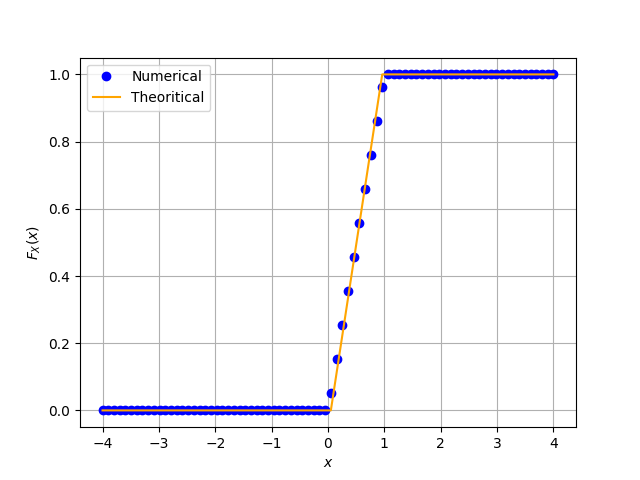
\includegraphics[width=\columnwidth]{./figs/1-2}
\caption{The CDF of $U$}
\label{fig:uni_cdf}
\end{figure}
\item
Find a  theoretical expression for $F_{U}(x)$.\\
\solution\\

The CDF of $U$ is given by
		\begin{align}
			F_U(x) = \pr{U \leq x} = \int_{-\infty}^{x}p_U(u)du
		\end{align}
We now have three cases:
		\begin{enumerate}
			\item $x < 0$: $p_X(x) = 0$, and hence $F_U(x) = 0$.
			\item $0 \leq x < 1$: Here,
				\begin{align}
					F_U(x) = \int_{0}^{x}du = x
					\label{eq:cdf-uni}
				\end{align}
		%	\item $x \geq 1$: Put $x = 1$ in \eqref{eq:cdf-uni} as $U$ is uniform in [0, 1] to get $F_U(x) = 1$.
		\item for $x>1$   $F_U(x)=1$
		\end{enumerate}
Therefore,
		\begin{align}
			F_U(x) = 
			\begin{cases}
				0 & x < 0 \\
				x & 0 \leq x < 1 \\
				1 & x \geq 1
			\end{cases}
			\label{eq:cdf-ans}
		\end{align}
		
\item
The mean of $U$ is defined as
%
\begin{equation}
E\sbrak{U} = \frac{1}{N}\sum_{i=1}^{N}U_i
\end{equation}
%
and its variance as
%
\begin{equation}
\text{var}\sbrak{U} = E\sbrak{U- E\sbrak{U}}^2 
\end{equation}

Write a C program to  find the mean and variance of $U$. \\
\solution Download the following files 
\begin{lstlisting}
we get https://github.com/pettugadipranav/Randomvar/blob/main/codes/1-4.c
we get https://github.com/pettugadipranav/Randomvar/blob/main/codes/cfunc.h
\end{lstlisting}
execute them using following files
\begin{lstlisting}
$ gcc 1-4.c
$ ./a.out
\end{lstlisting}
The value of mean is 0.500007\\
the value of variance is  0.083301\\
\item Verify your result theoretically given that
\begin{equation}
E\sbrak{U^k} = \int_{-\infty}^{\infty}x^k d F_{U}(x)
\end{equation}
\solution we know that \\ 

\begin{align}
\text{var}\sbrak{U} &= E\sbrak{U - E\sbrak{U}}^2 \\
	&= E\sbrak{U^2} - \left(E\sbrak{U}\right)^2\\
	E\sbrak{U^2} &= \int_{-\infty}^{\infty}x^2dF_U(x) \\
	&= \int_{-\infty}^{\infty}x^2p_U(x)dx \\
	&= \int_{0}^{1}x^2dx = \frac{1}{3}
\end{align}
and
\begin{align}
	E\sbrak{U} &= \int_{-\infty}^{\infty}xdF_U(x) \\
	&= \int_{-\infty}^{\infty}xp_U(x)dx \\
	&= \int_{0}^{1}xdx = \frac{1}{2}
\end{align}
we know  mean $= E\sbrak{U}=0.5$ 
\begin{align}
	\text{var}\sbrak{U} &= E\sbrak{U - E\sbrak{U}}^2 \\
	&= E\sbrak{U^2} - \left(E\sbrak{U}\right)^2 = \frac{1}{3} - \frac{1}{4} = \frac{1}{12} \\
\end{align}

\end{enumerate}

\section{Central Limit Theorem}
%
\begin{enumerate}[label=\thesection.\arabic*
,ref=\thesection.\theenumi]

%
\item
Generate $10^6$ samples of the random variable
%
\begin{equation}
X = \sum_{i=1}^{12}U_i -6
\end{equation}
%
using a C program, where $U_i, i = 1,2,\dots, 12$ are  a set of independent uniform random variables between 0 and 1
and save in a file called gau.dat\\
\solution download following files
\begin{lstlisting}
we get https://github.com/pettugadipranav/Randomvar/blob/main/codes/2-1.c
we get https://github.com/pettugadipranav/Randomvar/blob/main/codes/cfunc.h
\end{lstlisting}
and execute them using below commands
\begin{lstlisting}
$ gcc 2-1.c
$ ./a.out
\end{lstlisting}

\item Load gau.dat in python and plot the empirical CDF of $X$ using the samples in gau.dat. What properties does a CDF have?\\
\solution The CDF of $X$ is plotted in Fig. \ref{fig:gauss_cdf} by downloading below file
\begin{lstlisting}
we get https://github.com/pettugadipranav/Randomvar/blob/main/codes/2-2.py
\end{lstlisting}
and executed using below commands
\begin{lstlisting}
$ python3 2-2.py
\end{lstlisting}
\begin{figure}[!h]
\centering
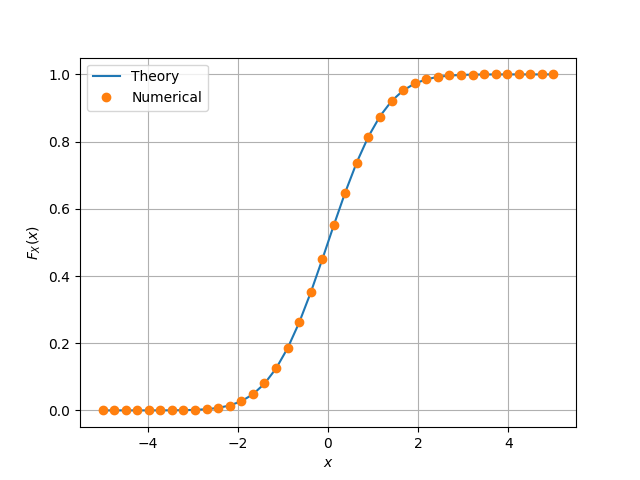
\includegraphics[width=\columnwidth]{./figs/2-2}
\caption{The CDF of $X$}
\label{fig:gauss_cdf}
\end{figure}
the properties of CDF are\\
1)The CDF is non decreasing function\\
2)It is symmetric about one point\\



\item
Load gau.dat in python and plot the empirical PDF of $X$ using the samples in gau.dat. The PDF of $X$ is defined as
\begin{align}
p_{X}(x) = \frac{d}{dx}F_{X}(x)
\end{align}
What properties does the PDF have?
\\
\solution The PDF of $X$ is plotted in Fig. \ref{fig:gauss_pdf} by downloading following codes
\begin{lstlisting}
we get https://github.com/pettugadipranav/Randomvar/blob/main/codes/2-3.py
\end{lstlisting}
and executed by using following commands
\begin{lstlisting}
$ python3 2-3.py
\end{lstlisting}
\begin{figure}[!h]
\centering
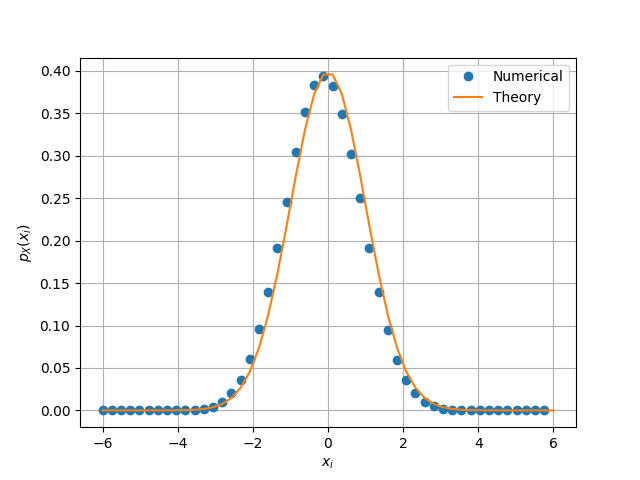
\includegraphics[width=\columnwidth]{./figs/2-3}
\caption{The PDF of $X$}
\label{fig:gauss_pdf}
\end{figure} 
some properties are\\
1)area under curve is 1\\ \\
2)it is symmetric about $x=\mu$\\ \\ 
3)it is increasing for $x<\mu$ and decreasing for $x>\mu$
\\ \\
\item Find the mean and variance of $X$ by writing a C program.\\
\solution to find mean and variance download following files
\begin{lstlisting}
we get https://github.com/pettugadipranav/Randomvar/blob/main/codes/2-4.c
we get https://github.com/pettugadipranav/Randomvar/blob/main/codes/cfunc.h
\end{lstlisting}
and execute them using following commands
\begin{lstlisting}
$ gcc 2-4.c
$ ./a.out
\end{lstlisting}
the value of mean is 0.000326\\
the value of variance is 1.000906\\

\item Given that 
\begin{align}
p_{X}(x) = \frac{1}{\sqrt{2\pi}}\exp\brak{-\frac{x^2}{2}}, -\infty < x < \infty,
\end{align}
repeat the above exercise theoretically.\\
\solution\\ 
1)CDF is calculated as follows :
\begin{align}
 & \int_{-\infty}^{\infty} \frac{1}{\sqrt{2\pi}}\exp\brak{-\frac{x^2}{2}} dx & \\
    & = \frac{1}{\sqrt{2\pi}} \times \sqrt{2\pi} & \\
     & = 1 &
\end{align}

MEAN can be calculated as follows :
\begin{align}
   & \int_{-\infty}^{\infty} x \times \frac{1}{\sqrt{2\pi}}\exp\brak{-\frac{x^2}{2}} dx& \\ 
   & = 0 &+
\end{align}
  
  2)mean is 
  \begin{align}
      E(x)&=\int_{-\infty}^{\infty} xp_x(x).dx\\
      &=\int_{-\infty}^{\infty} x\frac{1}{\sqrt{2\pi}}\exp\brak{-\frac{x^2}{2}}.dx\\
      &=0\\
  \end{align}
 E(x)=0\\ \\ \\
 
 3)VARIANCE can be calculated as follows :
 $var[x]=E[X^2]-E[X]^2$\\
 $var[X]=E[X^2]$
The variance is given by
		\begin{align}
		&	E\sbrak{X^2} = \int_{-\infty}^{\infty}x^2\frac{1}{\sqrt{2\pi}}\exp{\left(-\frac{x^2}{2}\right)} = 0 & \\
		& = \int_{-\infty}^{\infty} x \times x \frac{1}{\sqrt{2\pi}}\exp\brak{-\frac{x^2}{2}} dx & \\
		& = x\frac{1}{\sqrt{2\pi}}\exp\brak{-\frac{x^2}{2}}\Biggr|_{-\infty}^{\infty}& \\
 &+\int_{-\infty}^{\infty}1\times\int  \frac{x}{\sqrt{2\pi}}\exp\brak{-\frac{x^2}{2}}&\\
 & = x \times 0+\int_{-\infty}^{\infty}1 \times \int  \frac{x}{\sqrt{2\pi}}\exp\brak{-\frac{x^2}{2}} &\\
		&  = \frac{1}{\sqrt{2\pi}}\int_{-\infty}^{\infty} \exp\brak{-\frac{x^2}{2}} & \\
		& =1\\
		\end{align}
\therefore $var[X]=1$\\
\end{enumerate}


\section{From Uniform to Other}
\begin{enumerate}[label=\thesection.\arabic*
,ref=\thesection.\theenumi]
%
\item
Generate samples of 
%
\begin{equation}
V = -2\ln\brak{1-U}
\end{equation}
%
and plot its CDF.  \\
\solution download the following files
\begin{lstlisting}
we get https://github.com/pettugadipranav/Randomvar/blob/main/codes/3-1.c
we get https://github.com/pettugadipranav/Randomvar/blob/main/codes/cfunc.h
\end{lstlisting}
and execute them using following commands
\begin{lstlisting}
$ gcc 3-1.c
$ ./a.out
\end{lstlisting}
The CDF of V is plotted in Fig.  \ref{fig:3.1}  using following codes
\begin{lstlisting}
https://github.com/pettugadipranav/Randomvar/blob/main/codes/3-1.py
\end{lstlisting}
and execute them by following commands
\begin{lstlisting}
$ python3 3-1.py
\end{lstlisting}

\begin{figure}[!h]
\centering
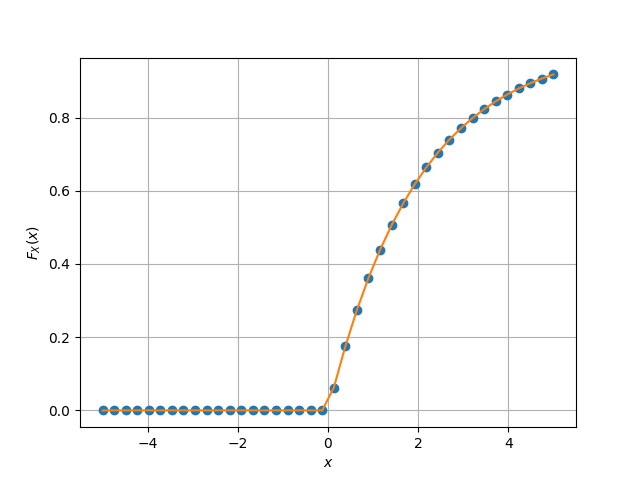
\includegraphics[width=\columnwidth]{./figs/3-1}
\caption{The CDF of $V$}
\label{fig:3.1}
\end{figure}
\item Find a theoretical expression for $F_V(x)$.\\
\solution
for$Y=G(X)$ then $F_Y(y)=F_X(G^-{}^1(y))$\\
$V=G(U)$
\begin{align}
   U&=G^-{}^1(V)\\
   &=1-e^-{}^\frac{V}{2}
\end{align}
then
   \begin{align}
    F_V(v)&=F_U(G^-{}^1(v))\\
    &=F_U(1-e^-{}^\frac{V}{2})
    \end{align}
    \begin{align}
     \implies F_V(v)&= 
			\begin{cases}
				0 & x < 0 \\
			1-e^-{}^\frac{V}{2} & x \geq 0
			\end{cases}
		\end{align}
\end{enumerate}
\solution
Note that the function 
		\begin{align}
			v = f(u) = -2\ln{(1 - u)}
		\end{align}
is monotonically increasing in [0, 1] and $v \in \mathbb{R^+}$. Hence, it is invertible and the inverse function is given by
		\begin{align}
			u = f^{-1}(v) = 1 - \exp{\left(-\frac{v}{2}\right)}
		\end{align}
		Therefore, from the monotonicity of $v$, and using \eqref{eq:cdf-ans},
		\begin{align}
			F_V(v) &= F_U\left(1 - \exp{\left(-\frac{v}{2}\right)}\right) \\
			\implies F_V(v) &= 
			\begin{cases}
				0 & v < 0 \\
				1 - \exp{\left(-\frac{v}{2}\right)} & v \geq 0
			\end{cases}
			\label{eq:f-v}
		\end{align}
		




\end{document}